\documentclass[a4paper,
               %boxit,
               %titlepage,   % separate title page
               %refpage      % separate references
              ]{jacow}

\ifboolexpr{bool{xetex} or bool{luatex}} % test for XeTeX/LuaTeX
 {}                                      % input encoding is utf8 by default
 {\usepackage[utf8]{inputenc}}           % switch to utf8

\usepackage{graphicx, subfigure}
\usepackage{booktabs}


\begin{document}
\title{BEAM COUPLING IMPEDANCE OF THE NEW BEAM SCREEN OF THE LHC INJECTION KICKER MAGNETS}
\author{H. Day\thanks{hugo.day@hep.manchester.ac.uk}, M.J. Barnes, F. Caspers, E. Métral, B. Salvant, J. Uythoven;  CERN, Switzerland}

\maketitle 


\begin{abstract}
The LHC injection kicker magnets experienced significant beam induced heating of the ferrite yoke, with high beam currents circulating for many hours, during operation of the LHC in 2011 and 2012. The causes of this beam induced heating were studied in depth and an improved beam screen implemented to reduce the impedance. Results of measurements and simulations of the new beam screen design are presented in this paper: these are used to predict power loss for operation after long shutdown 1 and for proposed HL-LHC operational parameters.
\end{abstract}

\section{Introduction}

The injection kicker magnets (MKIs) are fast pulsed transmission line kicker magnets, with a ceramic tube inserted into the ferrite yoke: this supports a number of screen conductors, designed to provide a good conducting path for the image currents of the circulating beam. One end of the screen is directly connected to the beam pipe whilst the other is capactively coupled to the beam pipe in order to preserve the fast field rise time of the magnet. The initial design foresaw using 24 equally spaced screen conductors, however poor HV performance necessitated that the 9 closest to the HV busbar be removed, leaving a large section of the ferrite yoke unscreened. During the 2011 and 2012 runs of the LHC, high temperatures were observed in several devices in the LHC, including the MKIs \cite{mki-heating}, which was attributed to beam induced heating. This heating was observed to raise the temperature of the ferrite yoke of one of the MKIs close to its Curie point during fills, thereby necessitating waiting times of several hours for the ferrite to cool before safe injection could be carried out \cite{mki-heating}. A magnet with an improved beam screen was inserted during technical stop 3 (TS3) (September 12), replacing the MKI8D which was measured to have the highest temperature \cite{mki-heatingTemp}; the replacement magnet was subsequently shown to have the lowest temperature of all injection kickers in the LHC.

Building on this success a new design has been proposed to satisfy competing needs of low rates of electrical breakdown, during magnet pulsing, and a low beam coupling impedance to reduce the power lost into the structure by wakefields; in addition to meeting strict requirements for magnet operation for field rise time and flat top ripple \cite{mkiUpgrade}. 

\begin{figure}
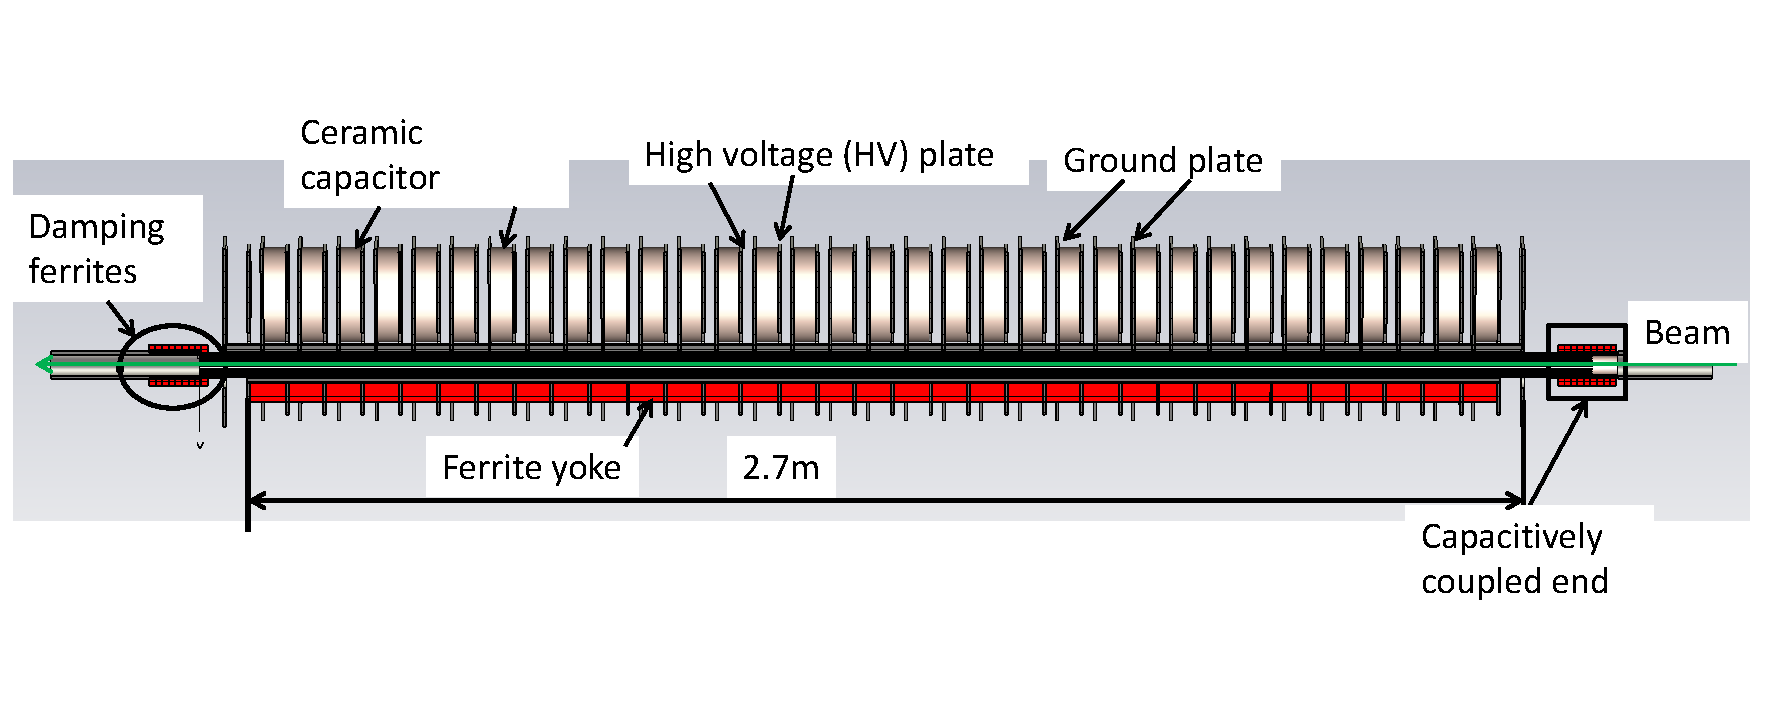
\includegraphics[width=0.5\textwidth]{TUPRI030f1.pdf}
\caption{Structure of the injection kicker magnets.}
\label{fig:mkiStruct}
\end{figure}

\section{New Beam Screen Design}

The new screen involves a redesign of the capacitively coupled end of the beam screen to reduce the electrical field, due to the induced potentials on the screen conductors during magnet pulsing. This reduced electric field decreases the possibility of surface breakdown on the internal face of the ceramic tube allowing additional screen conductors to be inserted, where previously they had been removed due to being located in regions of high electric field, providing complete screening of the ferrite yoke of the magnet. See \cite{mki-ElecBreakdown} for more information on behaviour relating to surface flashover. 

\begin{figure}
\begin{center}
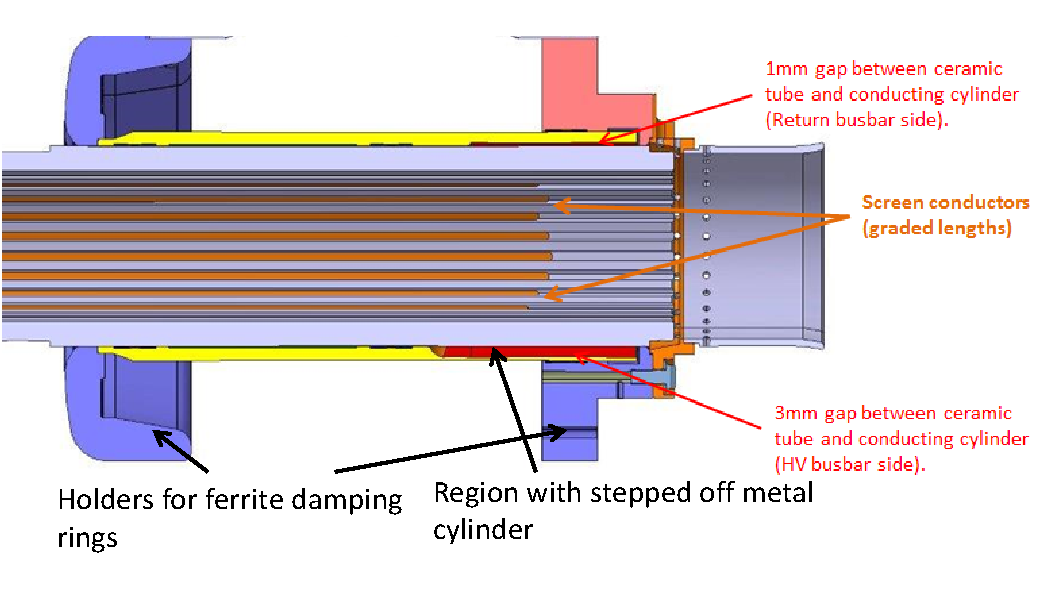
\includegraphics[width=0.5\textwidth]{TUPRI030f2.pdf}
\caption{Cross section of the new beam screen design}
\label{fig:beamScreenCross}
\end{center}
\end{figure}



\section{Impedance Measurements}

In order to observe the effect of manufacturing tolerances between kicker magnets, and as part of the campaign to characterise the impedance of all devices placed into the LHC, each of the MKIs with the new beam screen has its longitudinal beam coupling impedance measured following assembly. These measurements are carried out using the resonant coaxial wire method \cite{DayThesis}, a measurement technique that turns the device under test (DUT) into a coaxial resonator with a weak external coupling. This permits very sensitive measurements of the impedance of the DUT to be made at the expense of poor frequency resolution.

The real component of the longitudinal beam coupling impedance of an example of the new design, as well as for an MKI before LS1 (with 15 screen conductors), and the MKI8D before TS3 (a twist existed in the ceramic tube exposing ferrite to the beam) and the replacement from TS3 (with 19 screen conductors) are shown in Fig.~\ref{fig:Imp241915}. It can be seen that the new design has a substantially lower beam coupling impedance over the majority of the frequency range, with the broadband impedance seen in the case of 15 screen conductors becoming resonant in nature at certain frequencies with 24 conductors. This is due to the improved screening of the ferrite yoke by having 24 screen conductors equally distributed around the ceramic tube as opposed to an arc of $\approx$135$^{\circ}$ left unscreened when only 15 screen conductors are in place. The twist in the ceramic tube exposing more ferrite clearly increases the beam impedance substantially.

\begin{figure}
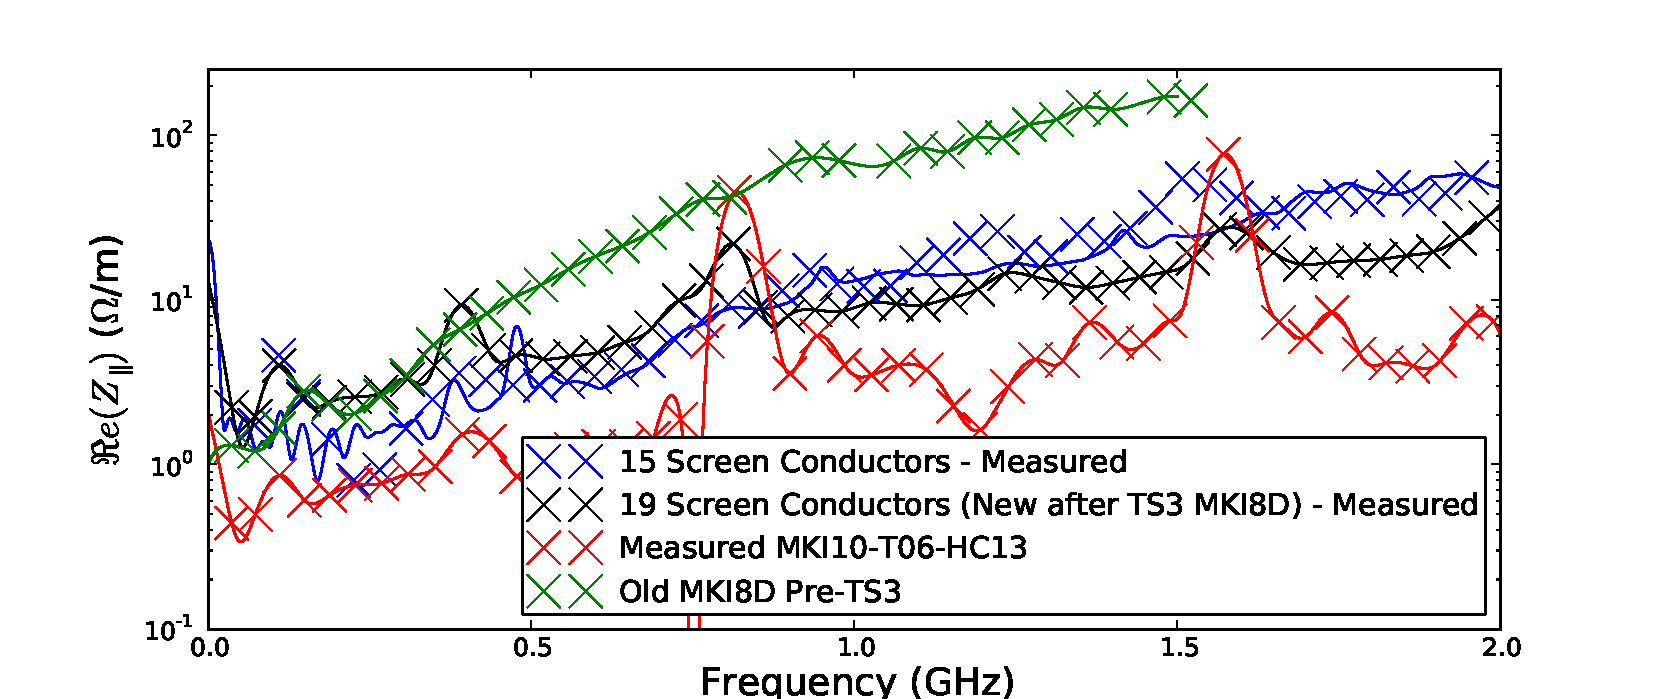
\includegraphics[width=0.5\textwidth]{TUPRI030f3.pdf}
\caption{The measured longitudinal beam coupling impedance for the new beam screen design, with 15 screen conductors, as was the case for most magnets prior to LS1, and the MKI8D pre and post TS3.}
\label{fig:Imp241915}
\end{figure}

Figure~\ref{fig:allNewMKIImp} shows the longitudinal impedance all 9 MKIs assembled with the new beam screen design to date (June 2014); the consistency between the magnets is very good up to the first measured resonance at 890~MHz. 

\begin{figure}
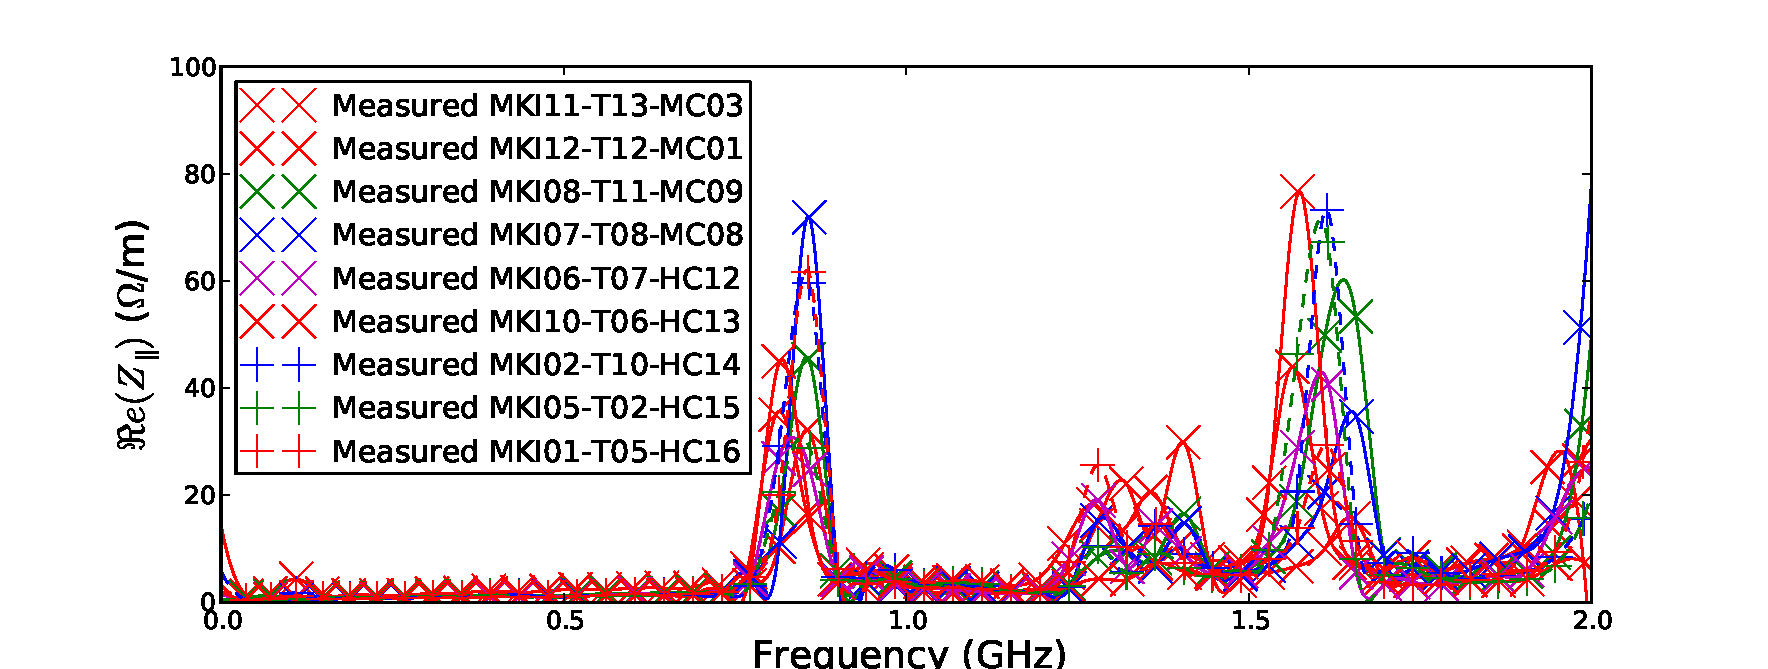
\includegraphics[width=0.5\textwidth]{TUPRI030f4.pdf}
\caption{The measured longitudinal beam coupling impedance for the first 9 magnets fitted with the new beam screen design.}
\label{fig:allNewMKIImp}
\end{figure}

It's known from simulations of the new design \cite{DayThesis} that a number of resonances are missed by the resonant coaxial wire method. It provides very good accuracy for the measurements but relatively poor frequency resolution; frequency data points are spaced such that $\Delta f \approx \frac{nc}{2L_{DUT}}$, where $n$ is an integer, $c$ the speed of light, and $L_{DUT}$ the length of the device measured. The classical coaxial wire technique gives an improved frequency resolution, however any residual mismatch in the characteristic impedance between the measurement network and the DUT will result in reflections in the system which limits the achieveable accuracy. It's also possible to use time domain gating to gate out reflected signals, however it's difficult to gate all reflections without losing sensitivity in the measurements.

A comparison of the beam coupling impedance for each method is shown in Fig.~\ref{fig:measComp}. The frequency domain data for the time domain gated measurement is processed to give a beam coupling impedance: it can be seen that there is a large DC offset, caused by the loss of transmitted energy by the gating of the signal. The resistively matched measurements give good results below $\approx$ 500 MHz but the residual mismatch in the system (characteristic impedance of DUT $Z_{c}^{DUT}\approx 270$~$\Omega$ was matched using a carbon film resistor of 220 $\Omega$) causes large oscillations which mask the true impedance. It can be seen that although the gated and matched network measurements give useful information, particularly the presence of lower frequency impedance, the absolute magnitude is not necessarily meaningful.

\begin{figure}
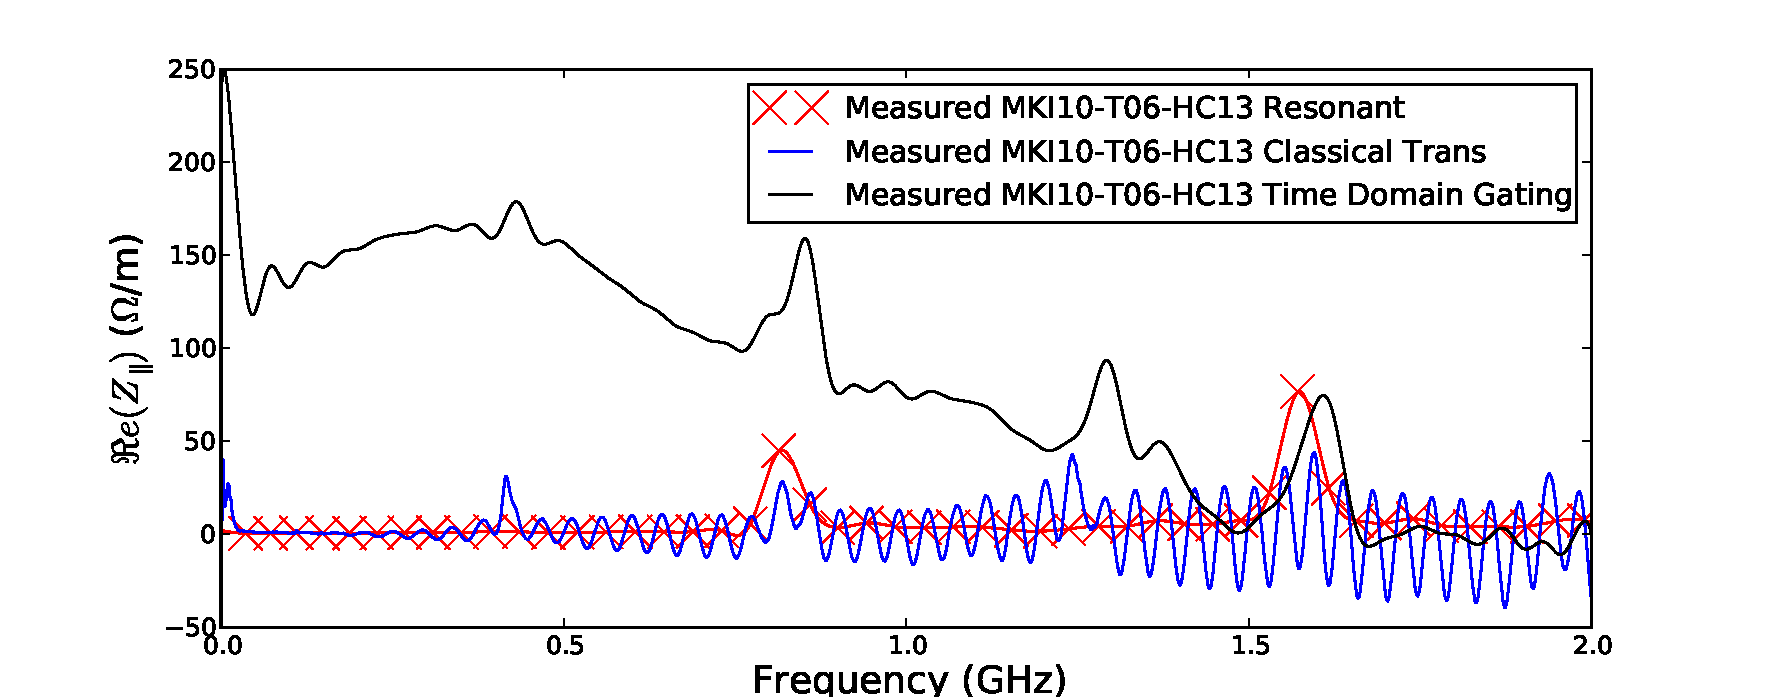
\includegraphics[width=0.5\textwidth]{TUPRI030f5.pdf}
\caption{The beam coupling impedance measurements for a magnet using either time domain gating only, or a matched resistor network in comparison to resonant coaxial wire measurements.}
\label{fig:measComp}
\end{figure}

\section{Power Loss}

To determine the temperatures reached during operation of the MKI under various operational conditions of the LHC it is necessary to calculate the power lost by the beam into the MKIs due to beam-wakefield interactions. Assuming $M$ equi-spaced, equal populated bunches in a circular machine, power loss is calculated using Eqn.~\ref{eqn:powLoss}, where $f_{0}$ is the revolution frequency, $\omega_{0}=2\pi f_{0}$, $e$ is the charge of an electron, $N_{b}$ is the number of particles per bunch, $\lambda(\omega)$ is the beam current spectrum, and $\Re{}e(Z_{\parallel}(\omega))$ is the real component of the longitudinal beam coupling impedance. $\lambda(\omega)$ is highly dependent on the bunch profile, especially the bunch length $t_{b}$. The bunch separation is defined by $\tau_{sep}$.

\begin{equation}
P_{loss} = 2 \left( f_{0} e M  N_{b}\right)^{2} \displaystyle\sum\limits_{n = -\infty}^{\infty}  \left| \lambda \left( p M \omega_{0} \right)  \right|^{2} \Re{}e \left[ Z_{\parallel} \left( p M \omega_{0} \right) \right]
\label{eqn:powLoss}
\end{equation}

The power losses are calculated assuming the parameters shown in Table~\ref{tab:beamPara}, representing the LHC operational parameters before long shutdown 1 (LS1), after LS1 and covering two  upgrade paths for High-Luminousity LHC (HL-LHC) using 50ns or 25ns bunch spacing. The power loss for 15 screen conductors (as most MKIs were prior to LS1) and with the new design with 24 screen conductors (as all MKIs will have post-LS1) is shown in Table~\ref{tab:powLoss}. The new beam screen design will dramatically reduction in the power lost into the MKIs, from 68~W pre-LS1 to between 34-52~W after LS1 - a reduction of 20-50\%. A range is given due to the variation between the MKIs with the new design. Tthe proposed HL-LHC parameters, with a higher beam current, will cause the power loss to increase significantly again - such that the power loss even exceeds the power loss experienced by the MKI8D before TS3 ($\approx$160~W) - indicating that heating may become a problem again if steps aren't taken to remedy the situation \cite{mkiCoolling}.

\begin{table}
\caption{Beam Parameters for different LHC operational modes}
\label{tab:beamPara}
\begin{center}
\begin{tabular}{c | c | c | c | c}
Mode & $\tau_{sep}$ (ns) & $N_{b}$ ($10^{11}$) & $ M $ & $t_{b}$ (ns) \\ \hline 
Pre-LS1 & 50 & 1.6 & $ 1380 $ & 1.2 \\ \hline 
Post-LS1 & 25 & 1.15 & 2808 & 1.0 \\ \hline 
HL-LHC, 50ns & 50 & 3.5 & 1380 & 1.0 \\ \hline 
HL-LHC, 25ns & 25 & 2.2 & 2808 & 1.0 \\ 
\end{tabular}
\end{center}
\end{table}

\begin{table}
\caption{Power Loss for different beam screen arrangements with different beam parameters (see Tab.~\ref{tab:beamPara}) in W/m}
\label{tab:powLoss}
\begin{center}
\begin{tabular}{c | c | c}
Mode & 24 screen cond. & 15 screen cond. \\ \hline 
Pre-LS1 & 20-35 & 68 \\ \hline 
Post-LS1 & 34-52 & 117 \\ \hline 
HL-LHC, 50ns & 151-240 & 538  \\ \hline 
HL-LHC, 25ns & 125-191 & 432  \\ 
\end{tabular}
\end{center}
\end{table}

\section{Future Plans}

\begin{figure}
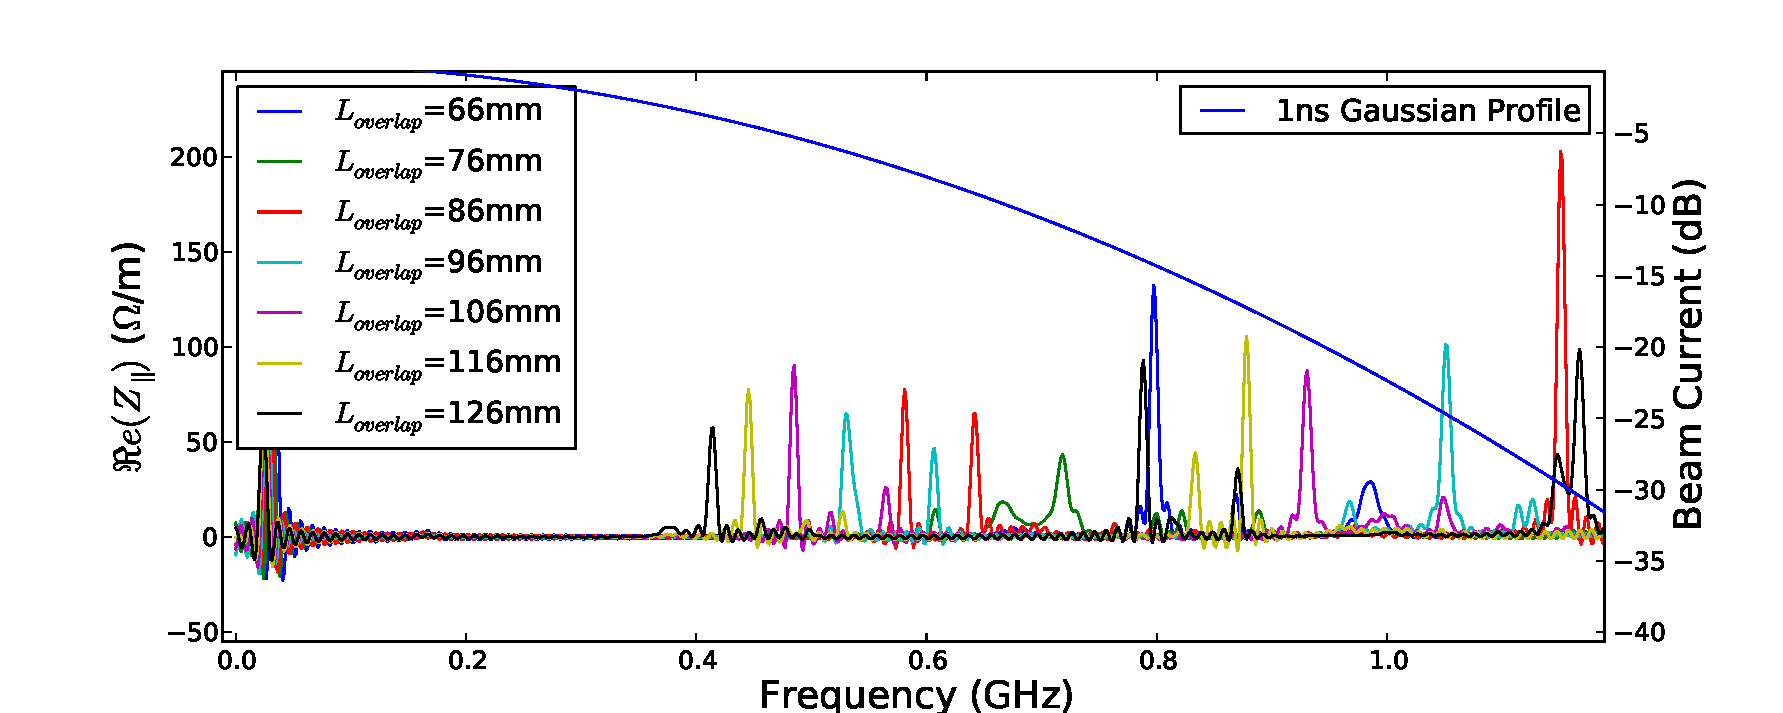
\includegraphics[width=0.5\textwidth]{TUPRI030f6.pdf}
\caption{The beam current spectrum of a 1ns Gaussian bunch compared to the real longitudinal beam coupling impedance for a number of different length overlaps.}
\label{fig:overLapSpec}
\end{figure}

Given the possibility of further heating problems in the MKIs under HL-LHC parameters, even with the new beam screen design, efforts are being made to increase the rate of power evacuation from the ferrite yoke by improving the ability of the magnet to radiate heat \cite{mkiCoolling}. In addition it's being considered how to further reduce the beam-induced power loss to the structure. If the ferrite yoke is well screened (as it is with the new beam screen design) the resonant impedance profile seen in Fig.~\ref{fig:allNewMKIImp} is determined by the overlap between the screen conductors and the external cylinder at the capactively coupled end, such that the resonant frequency $f_{res}$ is given by

\begin{equation}
f_{res} = \frac{n c}{2 \sqrt{\epsilon_{r}}\left( L_{overlap} + \delta_{fringe} \right)}
\end{equation}

where $\epsilon_{r}$ is the relative permitivitty of the ceramic tube, $L_{overlap}$ the length of overlap between the screen conductors and the external cylinder and $\delta_{fringe}$ the influence of the fringe fields on the effective length. It can be seen that by reducing the length of the overlap ($L_{overlap}=107$ mm maximum for the new design) it would be possible to reduce the interaction with the beam current spectrum as the resonances would be pushed to higher frequencies where the current spectrum is lower. Simulations have been carried out using CST particle studio \cite{cst-cite}, assuming different lengths of overlap, to verify that this path of investigation would be fruitful. Preliminary results (shown in Fig.~\ref{fig:overLapSpec}) indicate that the resonances indeed move to higher frequencies, however how these interact with the beam current spectrum in terms of power loss requires more investigation.

\section{Summary and Outlook}

The upgrades to the beam screen of the LHC injection kickers has been discussed from the view of the beam coupling impedance and beam-induced heating, demonstrating that there will be a substantially lower power loss into the magnets after LS1 is finished. The source of the high temperatures of MKI8D was found to be due to a twist in the ceramic tube, causing a power loss of $\approx$160 W, compared to 68 W for most magnets. Calculations for HL-LHC predict that heating of the device may again become a problem and solutions are discussed with preliminary results shown. In addition some comments on different beam impedance measurement methods are given relating to their use on low beam coupling impedance devices, including benefits and drawbacks in this situation.



\begin{thebibliography}{9}

\bibitem{mki-heating}
M.J. Barnes \emph{et al}., \emph{"Analysis of Measured Ferrite Heating of the LHC Injection Kickers and Proposals for Future Reduction of Temperature"}, IPAC'12, New Orleans, USA, 2012, TUPPR090.

\bibitem{mki-heatingTemp}
M.J. Barnes \emph{et al}., \emph{"Beam Induced Ferrite Heating of the LHC Injection Kickers and Proposals for Improved Cooling"}, IPAC'13, Shanghai, China, MOPWA031.

\bibitem{mkiUpgrade}
M.J. Barnes \emph{et al}., \emph{Upgrade of the LHC Injection Kicker Magnets}, IPAC'13, Shanghai, China, MOPWA030

\bibitem{mki-ElecBreakdown}
M.J. Barnes \emph{et al}., \emph{"Reduction of Surface Flashover of the Beam Screen of the LHC Injection Kickers"}, IPAC'13, Shanghai, China, MOPWA031.

\bibitem{mki-ElecBreakdown2014}
M.J. Barnes \emph{et al}., \emph{"High Voltage Performance of the Beam Screen of the LHC Injection Kicker Magnets"}, MOPME074, these proceedings.

\bibitem{DayThesis}
PhD Thesis, H. Day, 2013.

\bibitem{mkiCoolling}
M. Barnes \emph{et al}., \emph{"Cooling of the LHC Injection Kicker Magnet Ferrite Yoke: Measurements and Future Proposals"}, MOPME075, these proceedings.

\bibitem{cst-cite}
\texttt{http://www.cst.com}.

\end{thebibliography}
\end{document}

